\documentclass[Rapport/Rapport_main.tex]{subfiles}
\begin{document}
\subsection{Software Arkitektur}
\subsubsection{RPiApp}
I det følgende afsnit beskrives softwarearkitekturen for RPiApp. Den fulde dokumentation for arkiteturen kan ses i afsnit "XX" i bilaget "Systemarkitektur" \\
Softwareapplikationen består af forskellige sprog, men generelt er objektorienteret C++ benyttet. I forlængelse af dette, er der lavet en applikationsmdel til at beskrive strukturen og forløbet for applikationens objekt-orienteret softwaresystem. I de næste afsnit ses klasse-, sevkens og tilstandsdiagrammer for use case 1-4. \\\\
\textbf{Klassediagram for UC1 til UC4}\\
Traditionelt ville man udarbejde et klassediagram for hvert use case for systemet, men gennemstrømningen for systemet (Use cases) er en forlængelse af hinanden, overvejende use case 1 til 3. Figur \ref{fig:CD_RPI_RAP} viser klassediagrammet for UC1 til UC4
\begin{figure}[H]
    \centering
    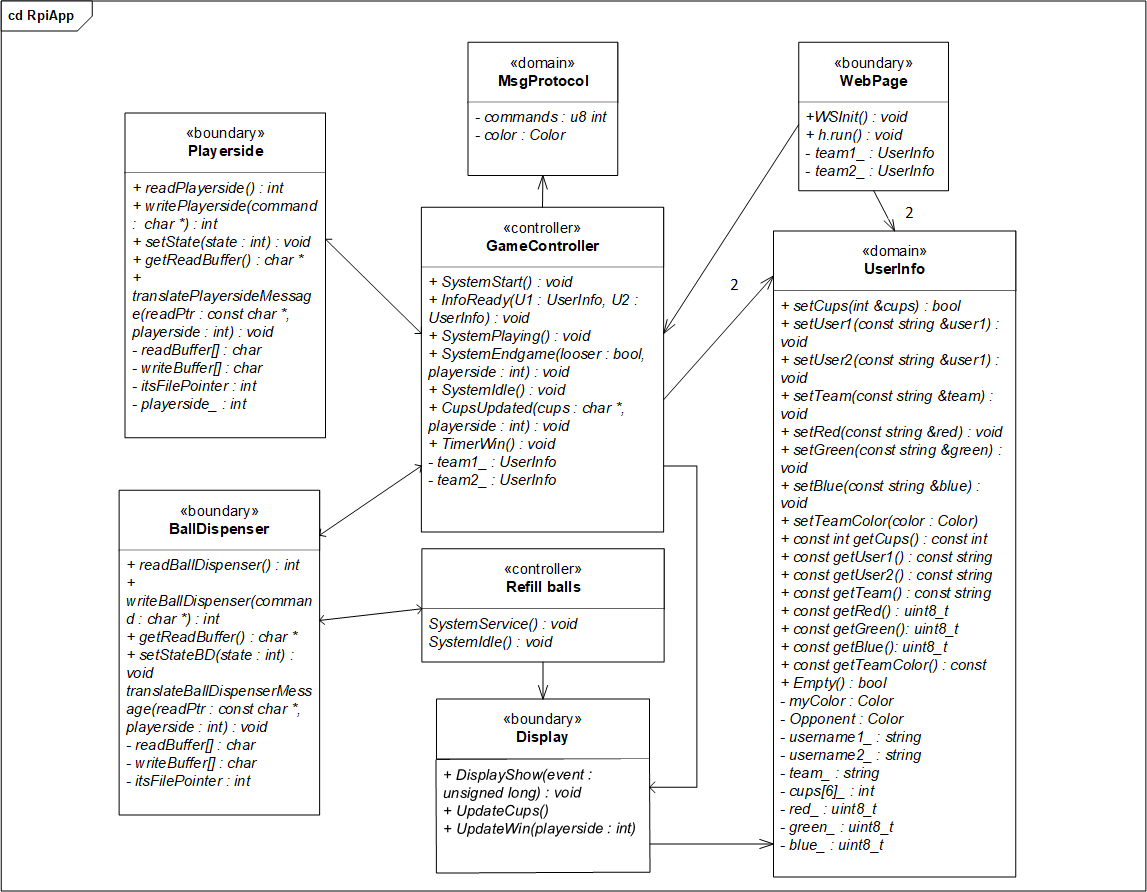
\includegraphics[width=\textwidth]{Arkitektur/Softwarearkitektur/Applikationsmodel/RPi/graphics_RPi/Class.png}
    \caption{Klassediagram for RPi}
    \label{fig:CD_RPI_RAP}
\end{figure}
\textbf{Controller:  GameController}\\
GameController er den centrale controller klasse for use case 1 - 3. Den sørger for at sende og modtage data gennem boundary klasserne Playerside og BallDispenser. Alt modtaget data bliver evalueret i GameController og sendt videre i overensstemmelse med protokollen og use case flow. Klassen varetager alt logikken og de flest beslutninger i systemet.\\\\
\textbf{Boundary:  PlayerSide}\\
Grænseflade til udveksling af data mellem RPi og Playerside-enhed. Klassen bruger filoperationer til at interagere med Kernal Space driveren - her søges for at omsætte en kommando modtaget fra en Playerside-enhed til MsgProtocol kommando, som kan behandles af GameController og vice versa.\\\\
\textbf{Boundary:  BallDispenser}\\
Grænseflade til udveksling af data mellem RPi og BallDispenser-enhed. Klassen bruger filoperationer til at interagere med Kernal Space driveren - her søges for at omsætte en kommando modtaget fra en BallDispenser-enhed til MsgProtocol kommando, som kan behandles af GameController og vice versa.\\\\
\textbf{Boundary: WebPage}\\
Klassen udgør serversiden af hjemmesiden. Den gør brug af et WebSocket API og står for at håndtere beskeder, som modtages fra client. Den skal initialisere to objektere af UserInfo klassen og sende dem til GameController klassen.\\\\
\textbf{Domain: UserInfo}\\
Klassen indeholder informationer, som repræsenterer Playersides (De fysiske spillersider). Klassen skal således indeholde alle informationer, som er relevante for et givet hold.\\\\
\textbf{Boundary: Display}\\
Boundary klassen Display repræsenterer den grafiske brugeroverflade. Den har til opgave at styre det fysiske display, som er koblet til RPi. \\\\
\textbf{Sekvensdiagram for UC1}\\
GameControlleren er logikken i systemet og tager alle de store beslutninger. Dens hovedfunktioner er at modtage data fra de enkelte delsystemer, som BallDispenser og Playerside, og agerer i forhold til dette. Boundary klasserne Playerside og BallDispenser læser konstant efter nyt data - når read-operationen kaldes, 'sover' processen indtil data er modtaget. Når nyt data er modtaget, behandles det og videresendes til GameController. \\\\
I forhold til spillets gang sender GameController information til delsystemerne via boundary klasserne. Fx sender den stadier til Playerside (IDLE) og BallDispenser (DISPENSE\_OFF). Den bruger to UserInfo objekter til at symboliserer to spillende hold, og kontrollere gennem dem, hvornår spillet er ovre (og andre informationer). \\\\
\begin{figure}[H]
    \centering
    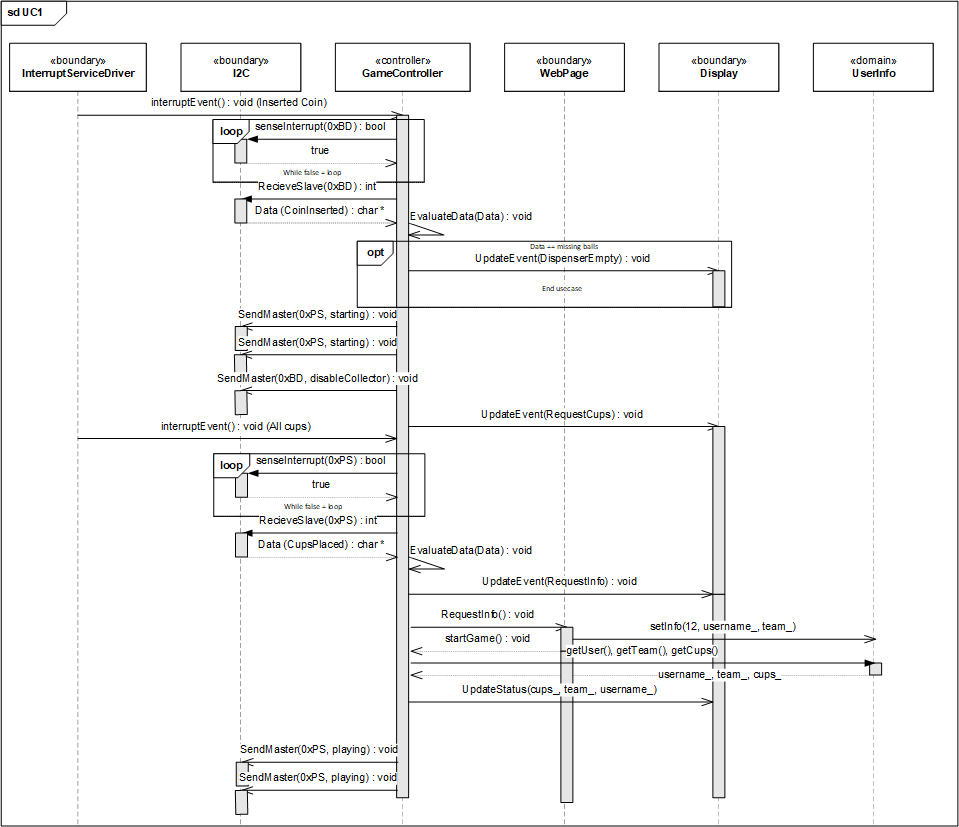
\includegraphics[width=\textwidth]{Arkitektur/Softwarearkitektur/Applikationsmodel/RPi/graphics_RPi/UC1_SD.png}
    \caption{Sekvensdiagram for UC1. Hver opmærksom på at mellemrummet mellem eksekverings specifikation 'boksen' indikerer en pause i processen; fx processeson 'sover', når der læses fra "BallDispenser" eller der ventes information fra WebPage}
    \label{fig:UC1_SD_RPi_RAP}
\end{figure}
Det kan ses på sekvensdiagrammet for UC1, at når funktionen readBallDispenser() eller readPlayerside() kaldes sover processen. Read og write operationerne i User Space er tilknyttet en Kernal Space driver. Device driveren er linket mellem det integrede hardware i Rasberry Pi W Zero og User Space applikationen - driveren beskrives kort i det næste afsnit. 

\subsubsection{i2c_interruptDriver}



\subsubsection{PlayersideApp}


\subsubsection{BallDispenserApp}
I dette avsnittet presenteres software arkitekturen for BallDispenser, for den fulle dokumentasonen refereres det til avsnitt 'XX' i Systemarkitektur bilaget. Applikasjonen er skrevet i C for å kunne kjøres på en PSoC. Under vil klasse, sekvens og tilstands diagrammene til UC1 og UC4 bli presentert.\\\\

\textbf{Sekvensdiagram for UC1}\\
\begin{figure}[H]
    \centering
    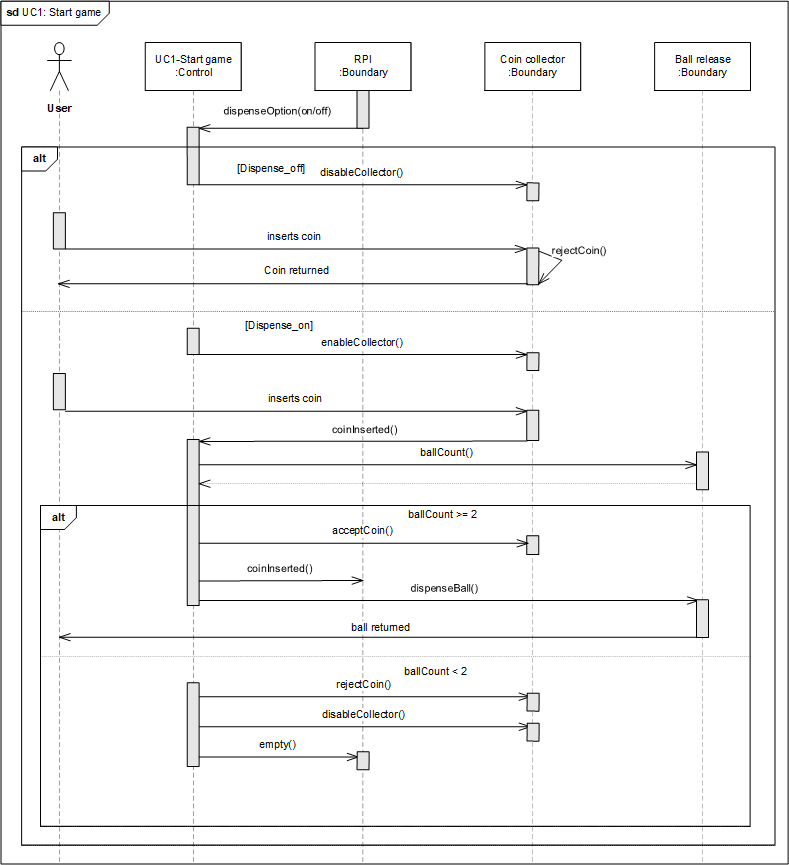
\includegraphics[width=\textwidth]{Arkitektur/Softwarearkitektur/Applikationsmodel/BallDispenser/graphicsBallDispenser/sdUC1.png}
    \caption{Sekvensdiagram for UC1 (Balldispenser)}
    \label{fig:BallDispScUC1}
\end{figure}

Ut fra sekvensdiagrammet (figur \ref{fig:BallDispScUC1}) kan vi se hvis en bruker innsetter en mynt i systemet mens det er i staten dispense\_off så kalder den rejectCoin() og fortsetter å vente. Mens hvis den er i dispense\_on skjekker den hvor mange baller som er igjen, hvis det det er nåkk akseperer den mynten, sender en beskjed til RPi og dispenserer baller. Hvis det ikke er nåkk avviser den mynten, disabler CoinCollector og sender beskjed til RPI.\\\\

\textbf{Sekvensdiagram for UC4}\\
\begin{figure}[H]
    \centering
    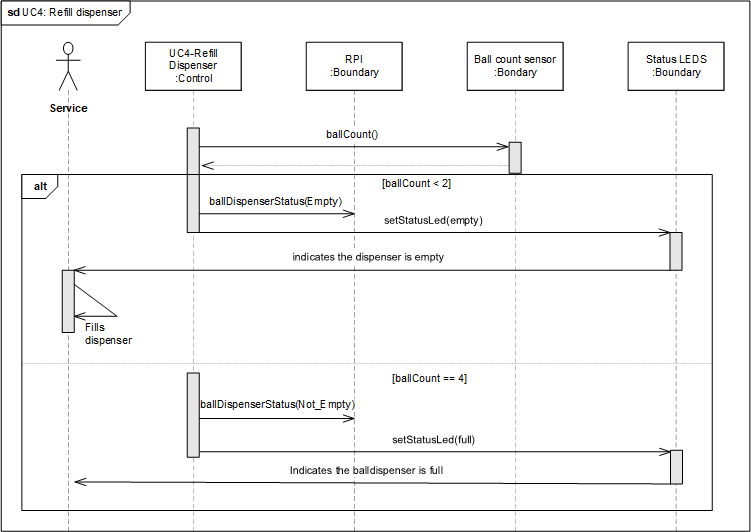
\includegraphics[width=\textwidth]{Arkitektur/Softwarearkitektur/Applikationsmodel/BallDispenser/graphicsBallDispenser/sdUC4.png}
    \caption{Sekvensdiagram for UC4 (Balldispenser)}
    \label{fig:BallDispScUC4}
\end{figure}

Ut fra sekvensdiagrammet (figur \ref{fig:BallDispScUC4}) kan vi se den starter med ballCount(), hvis den returnerer en verdi som er lavere enn 2 sender den beskjed til Rpien om at den er tom og indiker det til service medarbedidern ved å endre på status LEDene. Etter dispenseren har blitt fylt kalles ballCount() igjen og LEDene endres slik de viser dispenseren er full.

\end{document}